% !TeX program = pdflatex
% Corrected DC benchmark and validation experiments, October 2026.
\documentclass[sigconf,nonacm]{acmart}
\usepackage{amsmath,booktabs,tabularx,array}
\usepackage{xurl}
\setlength{\emergencystretch}{2em}
\newcolumntype{Y}{>{\raggedright\arraybackslash}X}
\graphicspath{{figures/}}
\setcopyright{none}
\settopmatter{printacmref=false}
\hypersetup{hidelinks,pdftitle={Heat-Aware Pedestrian Routing with Raster-Derived Exposure and Hard Detour Budgets: A Washington, DC Pilot},pdfauthor={Kameron Lee}}
% Generated by experiments/write_paper_results.py; do not hand-edit numerical results.
\newcommand{\ArtifactCommit}{aa4dd93ef1c0c970adebed22da1f7024b2a7c4dc}
\newcommand{\CommonCases}{2,000}
\newcommand{\CommonPairs}{500}
\newcommand{\AcceptedCount}{10,000}
\newcommand{\HeatRange}{0.92--0.96}
\newcommand{\DistanceRange}{4.84--6.55}
\newcommand{\BaselineH}{4.794}
\newcommand{\HeatReversalCount}{0}
\newcommand{\HeatReversalPct}{0.0}
\newcommand{\ShadowReversalCount}{26}
\newcommand{\ShadowReversalPct}{1.3}
\newcommand{\CompositeReversalCount}{1}
\newcommand{\CompositeReversalPct}{0.1}
\newcommand{\FallbackRange}{5.55--14.90}
\newcommand{\HeatCompositeWinner}{composite}
\newcommand{\HeatCompositeLoser}{UTCI-focused setting}
\newcommand{\HeatCompositeContrast}{0.009}
\newcommand{\HeatCompositeCI}{[$-0.015$, $0.035$]}
\newcommand{\HeatCompositeIntervalNote}{The interval includes zero.}
\newcommand{\HeatShadowWinner}{UTCI-focused setting}
\newcommand{\HeatShadowLoser}{direct-shadow setting}
\newcommand{\HeatShadowContrast}{0.028}
\newcommand{\HeatShadowCI}{[$0.010$, $0.045$]}
\newcommand{\HeatShadowIntervalNote}{}
\newcommand{\BudgetTwentyCases}{500}
\newcommand{\ExamplePair}{\texttt{od\_00000}}
\newcommand{\ExampleExtra}{13.1}
\newcommand{\ExampleReduction}{1.06}
\newcommand{\HigherHAtTwenty}{0}
\newcommand{\HeatWorseningSentence}{None has higher $H$ than its matched shortest route.}
\newcommand{\CompositeLowH}{0.705}
\newcommand{\CompositeLowExtra}{2.43}
\newcommand{\CompositeHighH}{1.137}
\newcommand{\CompositeHighExtra}{6.63}
\newcommand{\SensitivityAccepted}{1,600}
\newcommand{\DenseAccepted}{1,600}
\newcommand{\SensitivityPairs}{100}
\newcommand{\WeightChangeRange}{13--95}
\newcommand{\ThresholdLowChanged}{44}
\newcommand{\ThresholdLowDelta}{$-0.098$}
\newcommand{\ThresholdLowMagnitude}{0.098}
\newcommand{\ThresholdLowDirection}{higher}
\newcommand{\ThresholdHighChanged}{32}
\newcommand{\ThresholdHighDelta}{0.024}
\newcommand{\ThresholdHighMagnitude}{0.024}
\newcommand{\ThresholdHighDirection}{lower}
\newcommand{\SamplingFiveChanges}{78}
\newcommand{\SpacingMedian}{0.099}
\newcommand{\SpacingPninety}{0.252}
\newcommand{\ControlChanges}{0}
\newcommand{\RuntimeMedianRange}{0.180--0.729}
\newcommand{\RuntimePninetyRange}{0.702--2.459}
\newcommand{\RuntimeMaximum}{7.564}
\newcommand{\MainResultsTable}{\begin{table*}[t]
\caption{Matched outcomes on the same \CommonCases{} OD--budget cases. Positive $\Delta H$ and $\Delta J$ favor the environmental route; $\Delta S$ is added shade. Intervals resample whole OD pairs. Hybrid shade uses a different surrogate, so its comparison is omitted. Fallbacks are included.}
\label{tab:common}\centering\small
\begin{tabular}{@{}lrrrr@{}}\toprule
Method & Mean $\Delta H$ (K) [95\% interval] & Mean $\Delta J$ (K\,km) & Mean $\Delta S$ & Extra distance (\%)\\\midrule
Shortest & $0.000$ & $0.000$ & $0.000$ & $0.00$\\
Hybrid azimuth & $0.962$ [$0.911$, $1.016$] & $1.518$ & --- & $5.61$\\
Direct shadow & $0.922$ [$0.874$, $0.974$] & $1.352$ & $0.143$ & $6.55$\\
UTCI exceedance & $0.950$ [$0.900$, $1.004$] & $1.421$ & $0.139$ & $6.35$\\
Composite & $0.959$ [$0.907$, $1.013$] & $1.572$ & $0.139$ & $4.84$\\
\bottomrule\end{tabular}
\end{table*}}
\newcommand{\WeightResultsTable}{\begin{table}[t]
\caption{One-factor composite sensitivity on \SensitivityPairs{} complete paired paths, scored at 5 m and $26^\circ$C. Entries show removed/doubled coefficients. Positive $\Delta H$ means lower exceedance than the default.}
\label{tab:sensitivity}\centering\small
\begin{tabular}{@{}lrr@{}}\toprule
Coefficient & Changed paths & $\Delta H$ (K)\\\midrule
Thermal & 95/39 & $-0.580/0.050$\\
Shade & 18/17 & $-0.011/0.016$\\
Scenic & 43/36 & $-0.010/-0.008$\\
Traffic & 29/13 & $0.038/-0.018$\\
Slope & 19/13 & $-0.001/-0.028$\\
\bottomrule\end{tabular}
\end{table}}
\newcommand{\SamplingResultsTable}{\begin{table}[t]
\caption{Sampling disagreement with 5 m scoring of each same path, on \SensitivityPairs{} complete cases. Changes compare edge sequences with the 20 m default. The 5 m error is zero by construction.}
\label{tab:sampling}\centering\small
\begin{tabular}{@{}rrrr@{}}\toprule
Spacing (m) & Median error (K) & 90th pct. (K) & Changed\\\midrule
5 & 0.000 & 0.000 & 78\\
10 & 0.057 & 0.132 & 78\\
20 & 0.099 & 0.252 & 0\\
40 & 0.168 & 0.410 & 73\\
\bottomrule\end{tabular}
\end{table}}

\begin{document}
\title[Heat-Aware Pedestrian Routing]{Heat-Aware Pedestrian Routing with Raster-Derived Exposure and Hard Detour Budgets: A Washington, DC Pilot}
\author{Kameron Lee}
\email{2027klee@tjhsst.edu}
\affiliation{\institution{Thomas Jefferson High School for Science and Technology}\city{Alexandria}\state{Virginia}\country{USA}}

\begin{abstract}
Heat-aware walking routes trade modeled thermal exposure against extra distance. This pilot compares four environmental objective settings with shortest distance on a Washington, DC walking network, using Universal Thermal Climate Index (UTCI) and shadow rasters at one modeled hour. Five methods, 500 origin--destination pairs, and four distance allowances produce 10,000 routing attempts. On the \CommonCases{} cases shared by all methods, mean reductions in length-weighted UTCI exceedance above $26^\circ$C are \HeatRange{} K, with \DistanceRange{}\% extra distance. We evaluate both average exceedance and its length-scaled total, report capped-search fallback separately, and test weight, threshold, and sampling changes on a fixed 100-pair subset. Changing 20 m to 5 m sampling changes \SamplingFiveChanges{} of 100 paths. Exact-reference tests quantify losses from capped search on deliberately difficult generated graphs. Code, frozen input checksums, and route records are shared. The contribution is a reproducible comparison of objective choices within one solver. The study does not establish transfer beyond this snapshot or validate physiological benefit.
\end{abstract}
\keywords{pedestrian routing, UTCI, shade, detour constraints, computational benchmark}
\maketitle

\section{Introduction}
Two walking routes of similar length can have different shade and thermal conditions. A route that avoids exposed streets may reduce modeled heat exposure, but a long detour also adds walking. An explicit distance allowance makes this tradeoff understandable: a traveler can ask for a cooler route no more than 10\% longer than the shortest path.

This paper examines that formulation in a Washington, DC pilot. It attaches modeled UTCI and direct-shadow rasters to a pedestrian graph, then compares objectives that emphasize UTCI, shade, or a composite of environmental features. We study how these objective settings behave within one capped search implementation, using established hard-detour constraints and cost--distance labels.

The experiment uses 500 ordered origin--destination (OD) pairs, four detour allowances, and five methods. We compare routes on the same OD--budget cases and distinguish optimized routes from shortest-path fallback. We also test coefficient choices and sampling on a fixed subset, and check search outcomes against exact references on generated graphs.

The benchmark asks how much the selected objective changes modeled exceedance, added distance, and shade under a hard distance ceiling. It reports both average exceedance and an exceedance--distance index, because a cooler average can accompany more total walking through heat. The numerical results use a corrected rerun; the earlier archive is retained separately for audit.

\section{Related Work}
Shade-aware routing predates this study. Vartholomaios derives least-cost paths from SOLWEIG shadows \citep{vartholomaios2023}; Da et al. use image-derived shade \citep{da2024}; and Kolaxidis et al. incorporate solar exposure into pedestrian routing \citep{kolaxidis2025}. CoolWalks studies sunlit-distance penalties and the difference between centerline and detailed pedestrian networks \citep{wolf2025}. Yang et al. incorporate time-varying building shadows \citep{yang2025}, whereas this pilot holds the environmental field fixed.

Other work uses thermal indices. Colaninno et al. combine sidewalk mobility and microclimate modeling \citep{colaninno2025}. Patel et al. rank Google Maps candidate routes using SOLWEIG-GPU UTCI \citep{patel2026}. CoolPaths minimizes summed edge length times Physiological Equivalent Temperature (PET) under a detour limit \citep{verma2026}. Here, the primary reported metric is length-normalized UTCI exceedance. The routing formulation follows established resource-constrained shortest-path methods \citep{irnich2005}. More generally, Skoumas et al. enrich route computation with contextual information about places \citep{skoumas2015}; environmental attributes are another application of that idea.

UTCI converts meteorological and radiative conditions into an equivalent temperature under standardized reference assumptions \citep{brode2012}. SOLWEIG models urban radiation and mean radiant temperature \citep{lindberg2008}. Evidence that heat influences route choice \citep{basu2024} and that pedestrians seek shade \citep{levenson2025} motivates these routing preferences. It does not calibrate this paper's weights or validate its route-level outcomes for an individual pedestrian.

\section{Routing Pipeline}
\subsection{Graph and distance budget}
Let $G_0$ be the original directed walking multigraph. For a route $P$, let $L(P)=\sum_{e\in P}l_e$, where $l_e$ is edge length in metres. For an OD pair, define the original-network shortest distance $L_0^*$ and the final ceiling
\begin{equation}
 L_0^*=\min_{P\subset G_0} L(P),\qquad D_0=(1+\delta)L_0^*.
\end{equation}
The minimization is over directed paths connecting that pair. The allowance $\delta\in\{0.05,0.10,0.20,0.30\}$ limits proportional extra distance.

To reduce feature-extraction work, a node $v$ is retained when
\begin{equation}
 d_{G_0}(o,v)+d_{G_0}(v,d)\leq D_0+50\,\mathrm{m},
\end{equation}
where $d_G$ denotes shortest-path distance on graph $G$. The pipeline then assigns raster-backed features and removes edges lacking valid UTCI samples. The resulting feature graph is $G_f$. Network processing uses OpenStreetMap, OSMnx, and NetworkX \citep{osm2026,boeing2017,hagberg2008}.

\subsection{Sampling and reported exposure}
Each source segment in an edge geometry is subdivided to a maximum spacing of 20 m, retaining endpoints. Coordinates are transformed into each raster's coordinate reference system before sampling. Non-finite and NoData samples are omitted. Edges without UTCI samples are removed; edges without direct-shadow samples use the surrogate in Appendix~\ref{app:features}.

For UTCI samples $u_{ei}$ on edge $e$, define
\begin{align}
 \bar u_e&=\frac{1}{n_e^u}\sum_i u_{ei},\qquad u_e^{\max}=\max_i u_{ei},\\
 h_e&=\frac{1}{n_e^u}\sum_i\max(0,u_{ei}-\tau),\quad \tau=26^\circ\mathrm C.
\end{align}
For valid shadow samples $b_{ej}$, the direct-shade fraction is $s_e^{\rm dir}=(n_e^b)^{-1}\sum_j\mathbf1[b_{ej}\leq0.5]$; the raster convention is zero for shade and one for sun. Except for hybrid azimuth, each method uses this value when present and the surrogate $s_e^{\rm az}$ otherwise. The hybrid-azimuth method uses $s_e^{\rm az}$ everywhere.

The $26^\circ$C reference is the conventional UTCI boundary between no thermal stress and moderate heat stress \citep{eeautci}. It supplies an engineering reference rather than a personalized safety threshold. The main run uses a 20 m maximum interval on nominal 1 m rasters; Section~\ref{sec:sensitivity} compares alternative intervals against 5 m sampling on the same selected paths.

Reported route quantities are length-weighted edge summaries:
\begin{align}
 H(P)&=\frac{\sum_e l_eh_e}{L(P)},&\bar U(P)&=\frac{\sum_e l_e\bar u_e}{L(P)},\\
 S(P)&=\frac{\sum_e l_es_e}{L(P)},&U^{\max}(P)&=\max_e u_e^{\max}.
\end{align}
$H$ is mean positive UTCI exceedance, expressed in kelvins; $\bar U$ and $U^{\max}$ are UTCI values in degrees Celsius. $S$ is a shade fraction. Because sampling restarts at segment boundaries, these quantities are numerical proxies rather than uniform line integrals. As a post hoc check of normalization, we also calculate $J(P)=L(P)H(P)$, an exceedance--distance index in K\,m. It tests whether a lower route average offsets added distance. Neither $H$ nor $J$ is a validated physiological dose.

\subsection{Objectives and method variants}
We define the composite cost as an engineering score. It combines distance and time with thermal, scenic, traffic, and slope penalties; Appendix~\ref{app:cost} specifies the terms and normalizations. All are nonnegative. The thermal term is
\begin{equation}\label{eq:thermal}
 \phi_e=\frac{[\bar u_e-\tau]_+}{8\,\mathrm K}+\frac{[u_e^{\max}-\tau]_+}{10\,\mathrm K}+\frac{h_e}{6\,\mathrm K}+0.45(1-s_e),
\end{equation}
where $[x]_+=\max(0,x)$. Its correlated UTCI and shade components can count related radiative information more than once. Neither its coefficients nor the contextual proxies are fitted to route-choice or physiological observations.

Table~\ref{tab:methods} defines the four objective variants of this implementation. Distance and time remain active in all four. The focused methods are therefore not pure single-feature optimizations. For reporting, selected routes are evaluated with full features; the hybrid shade outcome remains a surrogate and is not comparable with direct shade.

\begin{table}[t]
\caption{Configured objective variants. $A_e$ is the distance--time term in Appendix~\ref{app:cost}; all environmental penalties also use its edge-length scale.}
\label{tab:methods}
\small
\begin{tabularx}{\columnwidth}{@{}lY@{}}\toprule
Method & Selection objective \\\midrule
Shortest & Dijkstra search minimizing $L(P)$.\\
Hybrid azimuth & $A_e$ plus twice the thermal term, using $s_e^{\rm az}$ on all edges.\\
Direct shadow & $A_e$ plus twice the shade-only part of $\phi_e$.\\
UTCI exceedance & $A_e$ plus twice the $h_e/(6\,\mathrm K)$ part of $\phi_e$.\\
Composite & Full thermal, scenic, traffic, and slope cost.\\\bottomrule
\end{tabularx}
\end{table}

\subsection{Capped search and fallback}\label{sec:search}
The solver first computes an unconstrained minimum-cost path and returns it if it meets $D_0$. Otherwise it explores cost--distance labels in increasing cost order. At a node, a label dominates another if it has no greater length and no greater cost. Labels are pruned when accumulated length plus shortest remaining distance exceeds $D_0$. Paths may not repeat nodes.

The dominance registry retains at most eight labels per node, ordered by cost then length. A newly queued label can survive even when omitted from that registry, so this does not bound the queue size. The label loop stops after 20,000 queue removals or 1.5 s, with timing beginning after the initial cost-path calculation. A capped search returns a feasible length-shortest fallback when available. If feature removal leaves no path within the original ceiling, the request fails. The final acceptance check enforces $L(P)\leq D_0$ within $10^{-6}$ m numerical tolerance.

We record whether a returned route came from the unconstrained cost path, label search, or shortest-path fallback, along with cap termination and failure type. The caps preclude a general optimality guarantee and do not bound end-to-end latency. Appendix~\ref{app:oracle} compares the search with exact enumeration on small graphs.

Before this rerun, the implementation was corrected to propagate the original-network ceiling, choose shortest parallel edges for shortest-path fallback, preserve sampled exceedance through objective projection, and use above-ground building heights. In particular, $\mathbb E[\max(0,U-\tau)]$ cannot be replaced with $\max(0,\mathbb E[U]-\tau)$. The earlier run lacked complete execution provenance; its records remain separate from the results below.

\section{Data and Analysis}
\subsection{Study domain and inputs}
The study uses one modeled Washington, DC snapshot labeled June 19, 2026, 14:00. The rerun explicitly uses UTC$-04{:}00$ for the hybrid solar calculation. Sustainable DC 2.0 reports a 13.3\% walking commute share in 2016 \citep{sustainabledc}; the sampled OD pairs nevertheless represent covered network nodes, not observed trips.

Table~\ref{tab:inputs} lists the input sources. SOLWEIG-GPU \citep{kamath2026} generated the nominal 1 m UTCI and shadow fields from urban-surface inputs and hourly Open-Meteo forcing \citep{zippenfenig2023}. These fields are held fixed and have no independent validation here. We recovered the versioned graph and rasters through Git LFS, recorded their SHA-256 checksums, and reproduced all 500 archived shortest distances exactly. The original graph has 61,543 nodes and 174,718 directed edges. For the hybrid proxy, building height is $\max(0,\mathrm{DSM}-\mathrm{DEM})$ on the aligned source grids; absolute surface elevation must not be interpreted as height above ground. Frozen routing inputs enable rerouting, but the retained provenance still lacks the forecast retrieval time, selected forecast model, and environmental-model release needed to regenerate the thermal field exactly.

\begin{table}[t]
\caption{Input layers. Different source years and street-centerline sampling limit spatial interpretation.}
\label{tab:inputs}
\small
\begin{tabularx}{\columnwidth}{@{}lY@{}}\toprule
Layer & Source and role \\\midrule
Walking network & OpenStreetMap via Geofabrik/OSMnx; directed centerlines, not verified sidewalks \citep{osm2026,boeing2017}.\\
UTCI and shadow & SOLWEIG-GPU modeled snapshot; thermal and direct-shade features \citep{kamath2026}.\\
Terrain/buildings & NOAA-hosted DC OCTO 2022 LiDAR and DEM; grade and height proxies \citep{noaa2022a,noaa2022b}.\\
Canopy/land cover & LiDAR canopy heights and DC 2020 layers; greenery, water, and surrogate shade \citep{dcgis2020a,dcgis2020b}.\\
Traffic & DDOT 2023 AADT lines; normalized traffic proxy, not sound measurements \citep{ddot2023}.\\\bottomrule
\end{tabularx}
\end{table}

\subsection{OD sample and experimental design}
The original generator uses the largest weakly connected graph component, then retains endpoints with finite UTCI and shadow raster values. With seed 42, it samples 500 distinct ordered node pairs whose shortest network distances lie between 400 and 3,000 m. We reuse those exact pairs. Their shortest distances range from 412.9 to 2,998.9 m. Figure~\ref{fig:od} locates the endpoints and shows the network-distance distribution used for eligibility. Large parts of the District have no sampled endpoints, so these locations do not establish district-wide coverage. Both maps use EPSG:32618 and frozen DDOT/DC GIS roads and water for geographic context; those display layers do not enter routing or exposure calculations \citep{ddotcontext2026,octowater2023}.

\begin{figure*}[t]
\centering
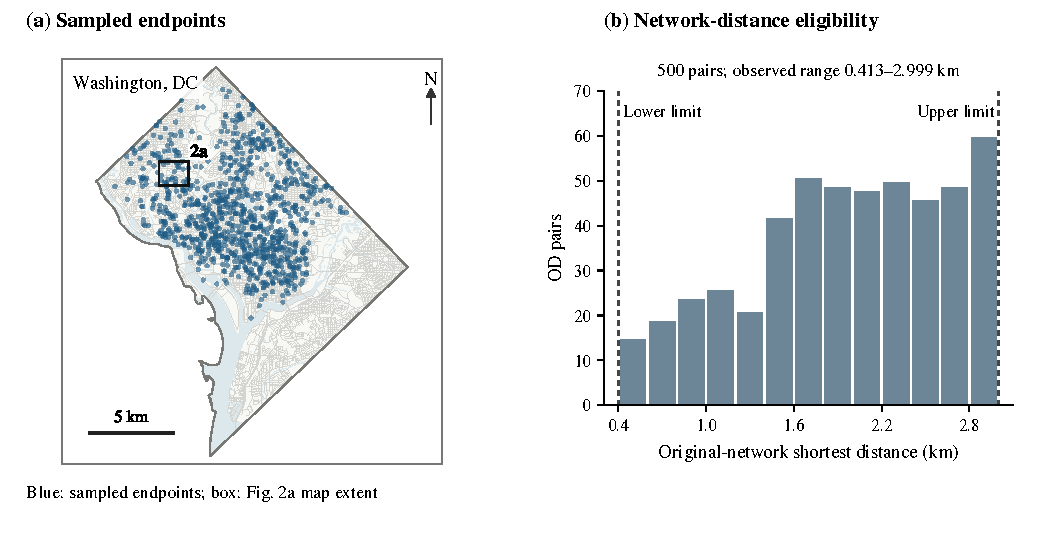
\includegraphics[width=\textwidth]{study_area.pdf}
\caption{Sample and distance eligibility. (a) Endpoint records for 500 OD pairs within the District; repeated endpoints can overlap. The box locates Figure~\ref{fig:route-cases}a. (b) Original-network shortest distances in 200 m bins, bounded by the 400--3,000 m sampling limits. Distances are network lengths, not straight-line separation.}
\Description{A contextual map of Washington DC with the sampled endpoints and example-route extents, alongside a histogram of the original 500 shortest network distances.}
\label{fig:od}
\end{figure*}

Each pair is evaluated with five methods at four allowances, giving 10,000 attempts. The 2,000 shortest-distance records repeat 500 pairs; the analysis checks their edge sequences across allowances. Environmental routes can change with allowance-specific corridors, features, and search. Records from the same OD pair are not independent observations. Eight deterministic shards assign pair index $i$ to $i\bmod8$, retaining every method and allowance for that pair. Each shard records its configuration, source-file hashes, and software versions. Timing includes corridor construction, feature extraction, and routing; direct-shadow methods share a persistent feature cache, while hybrid azimuth uses a separate cache.

\subsection{Matched comparison and uncertainty}\label{sec:matched-analysis}
Let $P^0_{i\delta}$ be the matched shortest route and $P^m_{i\delta}$ the route returned by method $m$. Positive improvements are
\begin{equation}
 \Delta H_{i\delta m}=H(P^0_{i\delta})-H(P^m_{i\delta}),
\end{equation}
with analogous $\Delta\bar U$; shade change reverses the order. Extra distance is $100(L(P^m_{i\delta})/L_0^*-1)$.

At each allowance, the primary comparison uses the intersection $\mathcal C_\delta$ of successful records for all five methods. Matching includes study, configuration hash, run identifier, raster timestamp, OD identifier, and allowance; duplicates are rejected. Shards retain their original identifiers, and matching stays within each shard. The common set contains \CommonCases{} of 2,000 pair--budget cases from \CommonPairs{} OD pairs. Pooled means weight these cases equally and include shortest-path fallbacks. We also count records with lower $H$ but higher $J$, using $10^{-9}$ K and $10^{-6}$ K\,m tolerances to exclude rounding noise.

For a paired method contrast, we compute the mean difference in recorded $H$ on the same common records. Percentile intervals use 2,000 bootstrap resamples of whole OD pairs, retaining each pair's available allowances, with seed 42. These exploratory 95\% intervals are not adjusted for multiple comparisons. They summarize variability within this one modeled snapshot and do not account for microclimate error or selection of the successful subset.

\subsection{Sensitivity design}\label{sec:sensitivity}
We use the first 100 serialized OD pairs at a 20\% allowance for 16 settings: the reference composite; removal and doubling of each of its thermal, shade, scenic, traffic, and slope coefficients; thresholds of 24 and $28^\circ$C; and maximum sample intervals of 5, 10, and 40 m. Each coefficient changes alone. Distance and time weights remain fixed. These exploratory choices test specific dependencies without fitting a preferred setting to the results.

Every selected path is rescored on the same unperturbed field with $\tau=26^\circ$C, first at 20 m and then at 5 m. Path changes use the ordered edge sequence. For a sampling setting, we compare its own $H$ with the 5 m score of that same path, separating metric disagreement from rerouting. The 5 m calculation is a denser numerical comparator, not ground truth or a proof of convergence at 1 m. Failures remain in the denominator, and dense-rescoring coverage is checked separately. The repeated reference setting also checks whether rerouting under the caps changes its own control path.

\section{Results}
\subsection{Feasibility and route sources}
The corrected run returns \AcceptedCount{} routes from 10,000 attempts, all within their original-network distance ceilings. Figure~\ref{fig:runtime}a separates the initial cost path, label-search result, and shortest-path fallback. Environmental fallback accounts for \FallbackRange{}\% of attempts across the four settings. These are feasible walking routes; fallback does not establish that a cooler route was found. The common comparison includes every such fallback.

The archived run accepted 6,093 of 8,000 environmental attempts and logged an expansion-limit error for each rejection. The corrected rerun records cap termination and returns a feasible fallback instead of treating that event as geographic infeasibility. Several implementation changes and an explicit solar-time offset separate the runs, so this comparison does not isolate the effect of any single fix.

\subsection{Exposure and added distance}
Table~\ref{tab:common} compares the same \CommonCases{} OD--budget cases for every method. Mean exceedance reductions range from \HeatRange{} K, with \DistanceRange{}\% extra distance. The shortest-route mean is \BaselineH{} K. The \HeatCompositeWinner{} has \HeatCompositeContrast{} K lower mean $H$ than the \HeatCompositeLoser{} (OD-cluster interval \HeatCompositeCI{} K). \HeatCompositeIntervalNote{} The \HeatShadowWinner{} has \HeatShadowContrast{} K lower mean $H$ than the \HeatShadowLoser{} (interval \HeatShadowCI{} K). \HeatShadowIntervalNote{}

\MainResultsTable

Figure~\ref{fig:route-cases} links one recorded route comparison with all \BudgetTwentyCases{} common pairs at a 20\% allowance. The mapped example adds \ExampleExtra{}\% distance and lowers $H$ by \ExampleReduction{} K. \HeatWorseningSentence{} Selection minimizes a sum of distance, time, and length-scaled thermal costs; it does not directly minimize the normalized $H$.

\begin{figure*}[t]
\centering
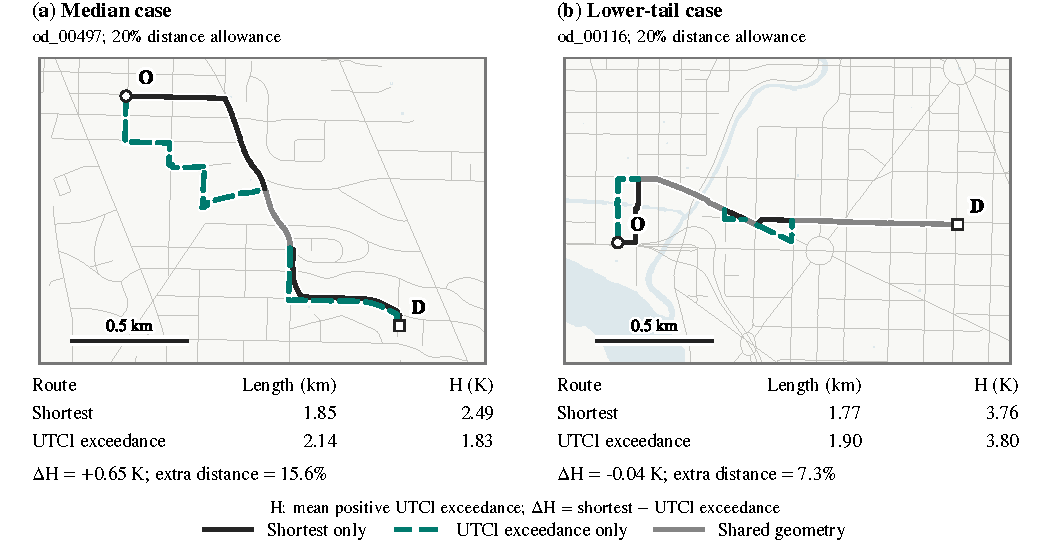
\includegraphics[width=\textwidth]{route_comparison.pdf}
\caption{Route change and paired outcomes at a 20\% distance allowance. (a) Recorded paths for \ExamplePair{}, selected by the median paired exceedance reduction. O/D denote origin/destination; gray segments are shared. (b) Every point is a common OD pair. Positive $\Delta H=H_{\rm shortest}-H_{\rm UTCI}$ means lower mean positive exceedance above $26^\circ$C. The outlined point identifies (a). Map coordinates use EPSG:32618.}
\Description{A street map comparing shortest and UTCI-exceedance paths, linked to the complete paired distribution of extra distance and exceedance reduction at the same allowance.}
\label{fig:route-cases}
\end{figure*}

Lower mean exceedance can accompany a higher exceedance--distance index. Direct shadow produces \ShadowReversalCount{} such records (\ShadowReversalPct{}\%). The composite has one such record; we find none for the UTCI setting. Table~\ref{tab:common} reports both $H$ and $J$. Hybrid shade uses a surrogate, so its $\Delta S$ is omitted; the raw records also report how much direct-shadow routing relies on surrogate fallback.

\subsection{Distance allowances}
For the composite, mean $\Delta H$ changes from \CompositeLowH{} K at a 5\% allowance to \CompositeHighH{} K at 30\%, with mean extra distance of \CompositeLowExtra{}\% and \CompositeHighExtra{}\%, respectively. These summaries use the same matched OD pairs at each allowance. A larger ceiling expands the feasible path set on a fixed graph. The implementation also rebuilds its corridor and applies caps, so the returned route need not improve monotonically for an individual pair.

\begin{figure*}[t]
\centering
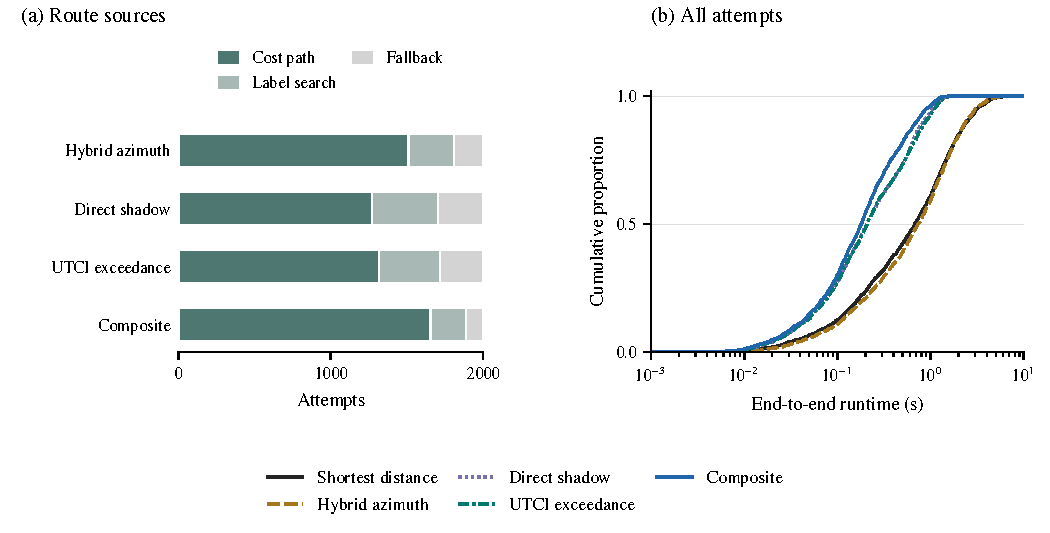
\includegraphics[width=\textwidth]{runtime_ecdf.pdf}
\caption{Returned-route sources and end-to-end runtime. (a) Environmental attempts split into the initial cost path, label search, and shortest-path fallback. (b) Empirical cumulative runtime distributions include all attempts for every method. The logarithmic time axis includes the full observed tails.}
\Description{A stacked bar chart of route-source counts for the four environmental settings and empirical runtime distribution curves for all five methods.}
\label{fig:runtime}
\end{figure*}

\subsection{Weights, threshold, and sampling}
All 1,600 sensitivity attempts succeed, and every selected path has 5 m rescoring. Table~\ref{tab:sensitivity} shows the one-factor weight changes. Removing or doubling a coefficient changes \WeightChangeRange{} of \SensitivityPairs{} common paths, depending on the coefficient. All exposure contrasts in that table use $\tau=26^\circ$C and 5 m samples, so the numbers reflect selected paths rather than changed reporting definitions.

\WeightResultsTable

Changing the selection threshold to 24 and $28^\circ$C changes \ThresholdLowChanged{} and \ThresholdHighChanged{} paths, respectively. On the common 5 m reporting field, mean $H$ is \ThresholdLowMagnitude{} K \ThresholdLowDirection{} than the default at $24^\circ$C and \ThresholdHighMagnitude{} K \ThresholdHighDirection{} at $28^\circ$C. These results quantify sensitivity to two nearby references; they do not calibrate a personal heat-stress threshold.

\SamplingResultsTable

Table~\ref{tab:sampling} compares sampling intervals on the same selected paths. At 20 m, the median absolute difference from 5 m is \SpacingMedian{} K and the 90th percentile is \SpacingPninety{} K. Switching to 5 m changes \SamplingFiveChanges{} of 100 paths, so the 20 m choice is not stable at the route level. The repeated reference returns identical paths.

\subsection{Observed runtime}
Figure~\ref{fig:runtime}b shows every attempt, including every fallback. Method medians range from \RuntimeMedianRange{} s; 90th percentiles range from \RuntimePninetyRange{} s. The complete observed maximum is \RuntimeMaximum{} s. These are end-to-end measurements from the rerun, including corridor and feature extraction, with shared caches and a fixed method order within each shard. Cache state, concurrent jobs, and host differences prevent a controlled solver-speed ranking. The 1.5 s cap applies only to the label loop.



\section{Discussion and Limitations}
The experiment compares engineering objectives within one search implementation. The fixed cohort and explicit fallback records make their outcomes directly comparable, but do not compare independent routing algorithms. The exact checks expose cap-induced losses even on 33-node networks (Appendix~\ref{app:oracle}); no optimality gap is available for the DC requests. A city-scale comparison with an exact or tightly bounded constrained-path solver remains necessary before claiming search quality.

The spatial and temporal scope is one modeled DC hour. The study cannot establish transfer across cities, seasons, neighborhoods, or times of day, and the fixed field ignores changes during a walk. The OD sample targets covered network nodes rather than observed demand. It therefore cannot estimate population benefits or typical pedestrian trips.

Street centerlines may lie in sun while a sidewalk is shaded, or the reverse. Source layers have different vintages; the traffic join uses a nearest-midpoint proxy in geographic coordinates without a maximum distance. Canopy does not guarantee shade at the pedestrian's position. Hybrid shade mixes geometry with cool UTCI samples and lacks independent shadow validation.

The composite remains uncalibrated. Thermal terms overlap, scenic and traffic scores are proxies, and the uncertainty input is zero. The one-factor checks describe local sensitivity at one allowance; they do not identify optimal weights or cover interactions. The small differences between objective settings require denser rerouting before being treated as a stable ranking. Sampling checks within the same modeled field do not test its physical accuracy.

The study has no field transects, participant study, or health measurements. Mean exceedance and exceedance--distance can disagree, and neither establishes comfort, safety, or clinical benefit. Independent environmental measurements and sidewalk-level networks are needed to test whether the modeled route differences survive at pedestrian height and position.

\section*{Code and Data Availability}
The \href{https://github.com/kameronlee/Routing/tree/\ArtifactCommit}{public artifact snapshot} includes code, the exact OD pairs, compressed route records, source/input checksums, analysis scripts, and figure inputs. Git LFS stores the versioned graph and rasters. The README gives rerun and analysis commands. Manifests preserve each shard's configuration and the routing source hashes; the original execution environment and thermal-field generation are only partly documented. The archived run and joint-weight exploration are retained separately and do not enter the revised result tables.

\begin{acks}
Computations used George Mason University's Office of Research Computing resources, supported in part by National Science Foundation award 2018631.
\end{acks}

\bibliographystyle{ACM-Reference-Format}
\bibliography{references}

\appendix
\section{Exact Search Check}\label{app:oracle}
We generate 100 graphs in each of three families with seed 42: 17-node layered directed graphs (five layers of width three), nine-node cyclic directed graphs, and 11-node chains with two parallel edges per step. Edge lengths are 40--180 m; thermal and contextual features are generated numerical values. An independent depth-first enumerator retains every simple edge path, including parallel-edge choices. It shares the configured edge-cost function with the router, so this tests search rather than validating the cost model.

Three hundred graphs, four allowances, and UTCI/composite objectives give 2,400 reference cases. Of these, 1,395 have a constrained optimum strictly above the unconstrained optimum. With the wall-clock cap disabled, the default eight-label registry and 20,000-expansion limit match every reference within relative tolerance $10^{-8}$ and respect every distance ceiling. Removing the expansion cap with registry sizes one, eight, or 32 also matches all cases. A deliberately tight 20-expansion condition matches 1,687 of 2,400 cases; its capped fallbacks can be suboptimal. Frozen generated graphs, raw results, and the enumerator are shared. Agreement on these small graphs supplies no optimality bound for the DC network.

To activate the actual default cap, we also generate 25 chains with 32 binary parallel-edge choices: 33 nodes and $2^{32}$ possible paths each. Short edges have integer lengths of 40--70 m and exceedance of 8--12 K; longer edges add 10--50 m with exceedance of 0--4 K. An independent dynamic program retains minimum cost at every integer distance. Across 200 graph--objective--allowance cases, the default count limits match 50 exact references and truncate 150 searches. Mean relative cost gap is 42.3\%, with a maximum of 136.0\%. These deliberately difficult cases diagnose cap behavior; they do not estimate error on the DC network. Both checks disable the wall-clock cap.

\section{Engineering Feature Definitions}\label{app:features}
Let $\operatorname{clip}(x)=\min(1,\max(0,x))$. Canopy and land cover are sampled on the densified centerline; building height is additionally sampled at lateral offsets of one-half and one estimated street width.

Let $c_e$ be the fraction of canopy samples at least 2 m high; $k_e$ the mean canopy height divided by 12 m and clipped; $v_e$ the larger of canopy- and land-cover-derived greenery fractions; and $w_e$ the water fraction. The scenic proxy is
\begin{equation}
 g_e=\operatorname{clip}(0.60c_e+0.25k_e+0.10v_e+0.05w_e).
\end{equation}
For nearest-midpoint AADT $a_e$ and the traffic layer's maximum $a_{\max}$, the traffic proxy is $n_e=\log_{10}(a_e+1)/\log_{10}(a_{\max}+1)$. This is not a decibel scale.

For solar altitude $\alpha$, azimuth $\theta$, bearing $\beta_e$, and estimated street width $W_e$, define
\begin{equation}
 q_e(z)=\operatorname{clip}\!\left(\frac{z|\sin(\theta-\beta_e)|}{W_e\max(\tan\alpha,10^{-6})}\right).
\end{equation}
If explicit width is missing, $W_e=\max(4,3.2p_e)$ m for $p_e$ lanes, or 10 m if lane count is also missing. With mean and maximum canopy/building heights, use $z_e^c=\max(\bar z_e^c,0.5z_e^{c,\max})$ and $z_e^b=\max(\bar z_e^b,0.6z_e^{b,\max})$. The geometry shade proxy is
\begin{equation}
s_e^{\rm geom}=\operatorname{clip}\!\left(\max\{c_e,q_e(z_e^b),c_eq_e(z_e^c)\}\right),
\end{equation}
set to one below the horizon. For local fractional hour $t$,
\begin{align}
 \tau_c(t)&=[25.5+3.2\cos(2\pi(t-14)/24)]^\circ\mathrm C,\\
 s_e^{\rm cool}&=(n_e^u)^{-1}\sum_i\mathbf1[u_{ei}\leq\tau_c(t)],\\
 s_e^{\rm az}&=\max(s_e^{\rm cool},s_e^{\rm geom}).
\end{align}
At $t=14$, the cool threshold is $28.7^\circ$C. These coefficients define a hybrid surrogate, not a fitted shadow model.

\section{Composite Cost}\label{app:cost}
Let signed elevation change be $\Delta z_e$, grade $m_e=\Delta z_e/l_e$, and $r_e=10|m_e|+[\Delta z_e]_+/(25\,\mathrm m)$. Edge time is $t_e$, estimated as $l_e/(1.35\,\mathrm{m\,s^{-1}})$ when unavailable. With $\phi_e$ from Eq.~\ref{eq:thermal}, the default cost is
\begin{align}
 A_e&=0.15\frac{l_e}{1000\,\mathrm m}+0.20\frac{t_e}{600\,\mathrm s},\\
 C_e&=A_e+\frac{\max(l_e,1\,\mathrm m)}{100\,\mathrm m}\bigl[\phi_e+0.45(1-g_e)^2\nonumber\\
 &\hspace{31mm}+0.45n_e^2+0.35r_e+0.15\sigma_e\bigr],\\
 C(P)&=\sum_{e\in P}C_e.
\end{align}
All ratios are dimensionless. $\sigma_e=0$ throughout this experiment. The one-factor checks change the corresponding coefficients and shade multiplier separately. The 1 m floor prevents a zero environmental scale on a malformed zero-length edge. These formulas specify the engineering score used in the corrected rerun.
\end{document}
